\chapter{A 16-bit shallow water model}
\label{chap:shallow_water}

%% CONTRIBUTION
\small \paragraph{Contributions} This chapter is largely based on the following publications \footnote{with the following author contributions.
Conceptualisation: MK, PDD. Data curation: MK. Formal Analysis: MK. Methodology: MK. Visualisation: MK. Writing – original draft:
MK. Writing – review and editing: MK, PDD, TNP.}

\vspace{\baselineskip}
\indent M Klöwer, PD Düben, and TN Palmer, 2019. \emph{Posits as an alternative to floats for weather and climate models},
\textbf{CoNGA'19: Proceedings of the Conference for Next Generation Arithmetic}, Singapore,
\href{https://doi.org/10.1145/3316279.3316281}{10.1145/3316279.3316281}.

\indent M Klöwer, PD Düben, and TN Palmer, 2020. \emph{Number Formats, Error Mitigation, and Scope for 16-Bit Arithmetics
in Weather and Climate Modeling Analyzed With a Shallow Water Model}, \textbf{Journal of Advances in Modeling Earth Systems},
\href{https://doi.org/10.1029/2020MS002246}{10.1029/2020MS002246}.
\vspace{\baselineskip}
\hrule
\vspace{\baselineskip}
\normalsize

\paragraph{Abstract.} The need for high precision calculations with 64-bit or 32-bit floating-point arithmetic for weather and
climate models is questioned. Lower precision numbers can accelerate simulations and are increasingly supported
by modern computing hardware. This paper investigates the potential of 16-bit arithmetic when applied within a shallow
water model that serves as a medium complexity weather or climate application. There are several 16-bit number
formats that can potentially be used (IEEE half precision, BFloat16, posits, integer and fixed-point). It is evident that a
simple change to 16-bit arithmetic will not be possible for complex weather and climate applications as it will degrade model
results by intolerable rounding errors that cause a stalling of model dynamics or model instabilities. However, if the posit number
format is used as an alternative to the standard floating-point numbers the model degradation can be significantly reduced.
Furthermore, a number of mitigation methods, such as rescaling, reordering and mixed-precision, are available to make model
simulations resilient against a precision reduction. If mitigation methods are applied, 16-bit floating-point arithmetic can be used
successfully within the shallow water model. The results show the potential of 16-bit formats for at least parts of complex weather
and climate models where rounding errors would be entirely masked by initial condition, model or discretisation error.

\section{Introduction}

Predictions of weather and climate remain very difficult despite the use of the world's fastest supercomputers. Although the available
computational resources have vastly increased over the last decades, forecast errors remain and have several origins
\citep{Palmer2012,Palmer2015}. They can be categorised as initial and boundary condition errors, model errors and discretisation
errors. For instance, uncertainties in the observational data and their assimilation contribute to the errors in the initial conditions
\citep{Ghil1991}; discrepancies between the mathematical model and the real world cause model errors; and the finite spatial and
temporal resolution result in discretisation errors. The forecast error is in general a combination and respective contributions can be
different for different variables and forecast lead times \citep{Jung2010,Palmer2019a}. 64-bit double precision floating-point numbers
(Float64, \cite{IEEE1985} and section \ref{sec:floats}) are used by default for weather and climate models since the 1980s with the
rise of 64-bit computing. The Float64 format introduces rounding errors \citep{Higham2002} that are largely negligible compared
to the other mentioned sources of error.

Faster calculations and communication on computing architectures can be achieved with reduced-precision floating-point numbers,
with a trade-off between speed and precision, provided a hardware-accelerated implementation. Deep learning algorithms require
only low numerical precision \citep{Wang2018,Sun2020} but high computational performance. The recent boom of machine learning
applications increased the demand on hardware-accelerated reduced precision calculations, such that hardware developments
increasingly offer more flexibility on low-precision number formats. While 16-bit arithmetic was not available for use on commodity
supercomputing hardware in the past, today most hardware vendors offer the use of 16-bit formats, such as 16-bit half precision
floating-point numbers (Float16, \cite{IEEE2008} and section \ref{sec:floats}), on the next generation of hardware
\citep{Sato2020,Burgess2019}.

Graphic processing units (GPU) started to support Float16 for increased performance \citep{Markidis2018}. Google's tensor processing
units (TPU, \cite{Jouppi2017,Jouppi2018}) support the 16-bit BFloat16 format, a truncated version of 32-bit single-precision floats (Float32),
as this format is sufficiently precise for many deep learning applications \citep{Kalamkar2019,Burgess2019,Gupta2015}. The world's fastest
supercomputers have reached peak performances of 500 Petaflop/s ($10^{17}$
floating-point operations per second) according to \href{https://top500.org}{TOP500.org} \citep{Dongarra2011} with Float64 as of June 2021,
but peak performances with Float16 are already beyond the exascale milestone ($10^{18}$ flop/s, \cite{Kurth2018,Kudo2020a}).

A gained speed from low-precision calculations can free resources to increase the complexity and therefore the forecast skill in
weather and climate models \citep{Bauer2020}. The European Centre for Medium-Range Weather Forecasts reduces the runtime by
40\% but not the forecast skill in their forecast model when using almost entirely Float32 instead of Float64 \citep{Vana2017}. MeteoSwiss
profited similarly with Float32 in their forecast model \citep{Rudisuhli2013,Fuhrer2018}. For the European ocean model NEMO
\citep{Madec2017} a mix of 32-bit and 64-bit arithmetic is a promising approach to keep precision-critical parts in high precision while
increasing performance in others \citep{TintoPrims2019}.

Software emulators for other number formats than Float32 and Float64 are often used to investigate rounding errors caused by lower
precision formats \citep{Dawson2017}. Although emulators are considerably slower than hardware-accelerated formats, they allow a
scientific evaluation of the introduced errors without requiring specialised hardware \citep{Johnson2020}, such as FPGAs
\citep{Russell2017}. Unfortunately, the computational performance cannot be assessed with software emulators.

Reducing the precision raises questions of the bitwise real information content (see chapter \ref{chap:compression}). In simplistic chaotic
models only a minority of bits contain real information \citep{Jeffress2017}, providing an information theoretic argument for reduced-precision
calculations. Recent research covers reduced precision in floating-point arithmetic in parts of weather forecast models,
such as the dynamical core \citep{Duben2014,Thornes2017,Chantry2019,Hatfield2020}; physical parameterisations \citep{Saffin2020};
the ocean model \citep{TintoPrims2019}; the land-surface model \citep{Dawson2018}; data assimilation \citep{Hatfield2017,Hatfield2018}.
In contrast to these studies, in this chapter we will evaluate various 16-bit arithmetics, as other formats than floats have gained little
attention for weather and climate models. Options for reduced-precision approaches are discussed and we present ways to mitigate rounding errors.

Although floating-point numbers are the dominating number format in scientific computing, alternatives have been proposed
\citep{Gustafson2017a}. Posit numbers claim to provide more effective precision in algorithms of machine learning
and linear algebra \citep{Gustafson2017a,Langroudi2019,Chen2018}, compared to floats with the same number of bits.
Posits were initially tested in simplistic weather and climate simulations \citep{Klower2019a} -- research that is extended
here, providing a more thorough investigation of various 16-bit number formats.

Is 16-bit arithmetic useful within weather and climate models? Which 16-bit formats are most promising, and can model
simulations be made resilient against a reduction in precision to 16 bits? These questions are covered in this chapter.
We apply several types of 16-bit arithmetic and test their impact on the simulated dynamics in a shallow water model that
serves as a medium-complexity weather and climate application.

The chapter is structured as follows: Section \ref{sec:swm_methods} introduces the methods specific to this chapter, including
an introduction to the shallow water equations and their discretisation. Section \ref{sec:swm_physics} presents the results of
using various 16-bit arithmetic in the shallow water model and section \ref{sec:swm_discussion} summarizes and discusses
the results in this chapter.

\section{Methods}
\label{sec:swm_methods}

The methods are structured as follows: Section \ref{sec:swm_swm} introduces the shallow water equations and our
discretisation thereof. For 16-bit arithmetic it is important to scale and reorder the equations which is presented in 
section \ref{sec:swm_scale}. Section \ref{sec:swm_semilagrange} describes a semi-Lagrangian advection scheme
resilient to 16-bit arithmetic. The concept of mixed precision and reduced precision communication are explained
in section \ref{sec:swm_mixed} and \ref{sec:swm_comm}.

An extensive discussion of the number formats used in this chapter is found in section \ref{sec:numbers}.

\subsection{The shallow water model}
\label{sec:swm_swm}

The shallow water model used here is an updated version of the one used in \cite{Klower2019a}, and most details described
therein are also valid here. A vertical integration of the Navier-Stokes equations yields the shallow water equations, that can
be used to understand many features of the general circulation of atmosphere and ocean as well as some two-dimensional
non-linear interactions on shorter length and time scales \citep{Gill1982,Vallis2006}. The shallow water equations for the
prognostic variables velocity $\mathbf{u} = (u,v)$ and sea surface elevation $\eta$ are
\begin{subequations}
\begin{align}
\frac{\partial \mathbf{u}}{\partial t} &+ (\mathbf{u} \cdot \nabla) \mathbf{u} +
f\hat{\mathbf{z}} \times \mathbf{u} = -g\nabla \eta + \mathbf{D} + \mathbf{F} \\
\frac{\partial \eta}{\partial t} &+ \nabla \cdot (\mathbf{u}h) = 0.
\end{align}
\label{eq:swe}%
\end{subequations}
$\eta$ can be interpreted as pressure for the atmosphere \citep{Gill1982}. The shallow water system is forced with a zonal
wind stress $\mathbf{F}$. The dissipation term $\mathbf{D}$ removes energy on large scales (bottom friction, \cite{Arbic2008})
and on small scales (diffusion, \citep{Griffies2000}). The non-linear term $(\mathbf{u} \cdot \nabla) \mathbf{u}$ represents advection of
momentum. The term $f\hat{\mathbf{z}} \times \mathbf{u}$ is the Coriolis force and $-g\nabla \eta$ is the pressure gradient
force, with $g$ being the gravitational acceleration. Eq. \ref{eq:swe}b is the shallow water-variant of the continuity equation,
ensuring conservation of mass.

The shallow water equations are solved in the $(x,y)$-plane over the zonally periodic rectangular domain $L_x \times L_y$,
of size $2000\op{km} \times 1000\op{km}$. We associate $x$ with the zonal and $y$ with the meridional direction. The domain
is centred at 45N with the beta-plane approximation \citep{Vallis2006}. The boundary conditions are periodic in zonal direction
and no-slip at the northern and southern boundary. The layer thickness is $h = \eta + H(x)$, with
\begin{equation}
H(x) = H_0 - H_1\exp\left(-H_\sigma^{-2}(x-\tfrac{L_x}{2})^2\right)
\end{equation}
being the undisturbed depth, representing a meridional mountain ridge at $x=\tfrac{L_x}{2}$ spanning from the southern to
the northern boundary. The standard depth is $H_0 = 500\op{m}$. The ridge has a maximum height of $H_1 = 50\op{m}$
and a characteristic width of $H_\sigma = 300\op{km}$, which makes the zonal current barotropically unstable. The flow
regime is therefore governed both by eddy-mean flow as well as eddy-eddy interactions \citep{Ferrari2010}. The wind stress
forcing $\mathbf{F} = (F_x,0)$ is constant in time, acts only on the zonal momentum budget
\begin{equation}
Fx = \frac{F_0}{\rho h} \cos\left(\pi\left(y{L_y}^{-1} - 1\right)\right)^2
\end{equation}
and vanishes at the boundaries. The water density is $\rho = 1000\op{kg}\op{m}^{-3}$ and $F_0 = 0.12\op{Pa}$.
The wind forcing acts as a continuous input of large-scale kinetic energy that is balanced by the dissipation term.

The dissipation term $\mathbf{D}$ is the sum
\begin{equation}
\mathbf{D} = -\frac{c_D}{h}\| \mathbf{u} \| \mathbf{u} - \nu \nabla^4 \mathbf{u}
\label{eq:diss}
\end{equation}
of a quadratic bottom drag with dimensionless coefficient $c_D = 10^{-5}$ \citep{Arbic2008}
and a biharmonic diffusion with viscosity coefficient $\nu \approx 1.33\times10^{11} \op{m}^4\op{s}^{-1}$ \citep{Griffies2000}.

The shallow water equations are discretised using 2nd order centred finite differences on an Arakawa C-grid \citep{Arakawa1977}
and the fourth-order Runge-Kutta method \citep{Butcher2016} is used for time integration of the pressure, Coriolis and advective terms,
whereas a semi-implicit method is used for the dissipative terms $\mathbf{D}$. We present results of simulations with three different
levels of resolution: high resolution simulations with a grid spacing of $\Delta = 5\operatorname{km}$ (400x200 grid points), medium
resolution simulations with a grid spacing of $\Delta = 20\operatorname{km}$ (100x50 grid points) and low resolution with a
grid-spacing of $\Delta = 40\operatorname{km}$ (50x25 grid points). The grid spacing in $x$ and $y$-direction is always equal,
$\Delta x = \Delta y = \Delta$. The time step $\Delta t = 282\op{s}$ at $\Delta = 20\mathrm{km}$ is chosen to resolve surface gravity waves,
traveling at an estimated phase speed of $\sqrt{gH_0}$ with a CFL number close to 1 and gravitational acceleration $g=10\op{ms}^{-1}$.
The advection terms are discretised using an energy and enstrophy conserving scheme \citep{Arakawa1990,Salmon2004,Salmon2007}.

The shallow water equations are extended with an advection equation for tracers. Temperature and humidity or salinity are examples
of tracers in the atmosphere and the ocean. For simplicity, we regard them as passive here, such that they do not influence the flow.
The advection of a passive tracer $q$ given a velocity $\mathbf{u}$ is governed by
\begin{equation}
\frac{\partial q}{\partial t} + \mathbf{u} \cdot \nabla q = 0.
\label{eq:adv}
\end{equation}
A semi-Lagrangian advection scheme \citep{Smolarkiewicz1992} is used to discretise Eq. \ref{eq:adv}. In this discretisation, the tracer
concentration for a given grid cell, which is considered to be the arrival point, is calculated from the concentration at a departure point
at the previous time step. Starting from each arrival point, velocities are traced back to find the respective departure points. 
While the arrival points correspond to grid cells, the departure points in general do not coincide with the grid cells, such that an interpolation
is required. The concentrations at the surrounding grid points are bilinearly interpolated onto the departure point, which
is then used as the concentration at the arrival point one advective time step later.

\begin{figure}[htbp]
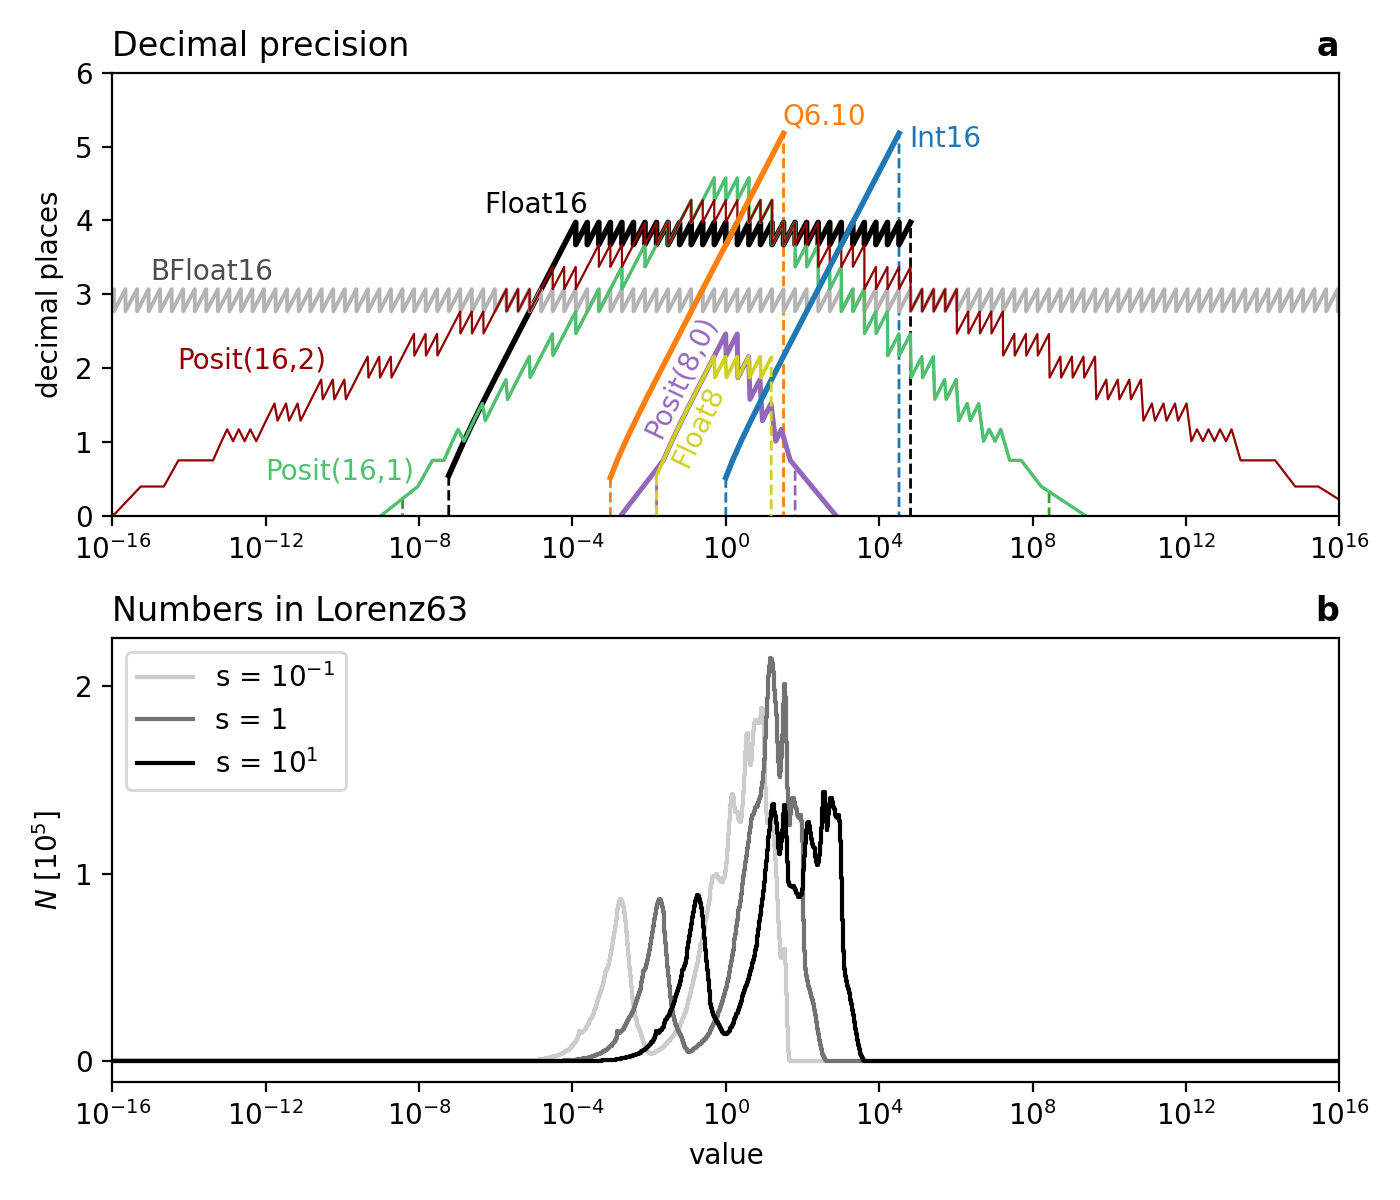
\includegraphics[width=1\textwidth]{Figures/swm/decimal_precision.png}
\caption{\textbf{Matching arithmetic results to the decimal precision of number formats.}
\textbf{a} Decimal precision for various number formats. Dashed vertical lines indicate for each format the range from $minpos$ to
$maxpos$ of representable numbers. Float64, Float32 and Posit32 are beyond the axes limits. \textbf{b} Histogram of results
of the absolute values of all arithmetic operations in Lorenz 1963 system rescaled by $s$ from \citep{Klower2019a}.}
\label{fig:swm_dec_prec}
\end{figure}

\subsection{Scaling and reordering the shallow water equations}
\label{sec:swm_scale}

Equations can be rescaled via multiplication with a constant rescaling factor $s$ to shift the dynamic range occurring in an algorithm
towards larger numbers (for $s > 1$) or towards smaller numbers ($s < 1$). Rescaling can be used to adjust the number range to the
decimal precision of the number formats (see section \ref{sec:decimal_precision}). If nonlinear terms are considered, this multiplicative
rescaling is ineffective, as the rescaling factor $s$ appears inside the non-linear terms. The nonlinear terms are therefore effectively
invariant under multiplicative rescaling and only the linear terms are scaled by $s$. Fig. \ref{fig:swm_dec_prec} includes histograms of
numbers occurring in the rescaled Lorenz system \citep{Lorenz1963,Kwasniok2014,Jeffress2017,Tantet2018} as an example
from \cite{Klower2019a}. For posit arithmetic it is preferable to use $s=\tfrac{1}{10}$ in the Lorenz system to scale the prognostic
variables to match the range of highest decimal precision around $\pm1$, which increases the complexity of the Lorenz attractor
and decreases the average rounding error.

Furthermore, it is sometimes possible to avoid intermediate arithmetic results, which may be outside the dynamic range of a number format,
by changing the order in which multiplications and divisions are executed. In general, it is preferable to combine such operations to a single
multiplication with a constant which can be precomputed. Although this will have a negligible effect on the rounding error for floating-point
arithmetic due to the approximately constant decimal precision throughout the range of numbers (subnormals excluded), it reduces the risk
of over or underflow (see also Fig. \ref{fig:a64fx_bitpatternhist} and chapter \ref{chap:hardware} in general).

The dynamic range of representable numbers with 16-bit arithmetic is for most formats discussed here considerably smaller than with
Float32 or Float64 (Table \ref{tab:formats}). It is therefore important to rescale the calculations to limit the range of arithmetic results to
stay within the bounds of a given 16-bit format.

The prognostic variables in the shallow water equations are typically $\mathcal{O}(1\op{ms}^{-1})$ for $\mathbf{u}$, $\mathcal{O}(1\op{m})$
for $\eta$ and $\mathcal{O}(1)$ for $q$ in the barotropic setup is used (section \ref{sec:swm_swm}). Their physical units are therefore retained
in the discretised numerical model and we do not apply a rescaling of the shallow water equations as a whole in this chapter. Chapter
\ref{chap:hardware} rescales the shallow water equations fully to avoid subnormals, which is discussed in more detail in section
\ref{sec:swm_scaling}.

In this chapter, however, we introduce dimensionless gradients as the grid spacing $\Delta$ in units of meter is large for geophysical flows.
We therefore use dimensionless Nabla operators $\tilde{\nabla} = \Delta\nabla$. The continuity equation Eq. \ref{eq:swe}b, for example,
reads then as
\begin{equation}
\eta^{n+1} = \eta^n + \tilde{\Delta t}\left( - \tilde{\nabla} \cdot (\mathbf{u}h)^n\right)
\label{eq:discr}
\end{equation}
for an explicit time stepping scheme. $\tilde{\Delta t}$ is the rescaled time step, a Runge-Kutta coefficient times $\tfrac{\Delta t}{\Delta}$ to
combine a division by a large value for $\Delta$ and a subsequent multiplication with a large value for $\Delta t$ into a single multiplication
with $\tilde{\Delta t}$. The other terms are rescaled accordingly ($\tilde{f} = f\Delta$; $\tilde{\mathbf{F}} = \mathbf{F}\Delta$). As these terms
remain constant, they can be precomputed at higher precision during model initialisation. The momentum equations are rescaled similarly.

Diffusion is an example of a discretization scheme that requires rescaling for the arithmetic results to fit into the limited dynamic range.
Biharmonic diffusion \citep{Griffies2000} calculates a fourth-derivative in space, which is with $\mathcal{O}(10^{-20})$ often very small in
geophysical applications, due to the large physical dimensions, when using meters as a unit for length. Contrarily, biharmonic viscosity
coefficients are typically very large
$\mathcal{O}(10^{11})$.
We therefore rescale $\mathbf{D}$ accordingly
\begin{equation}
\tilde{\mathbf{D}} =-\frac{\tilde{c_D}}{h}\| \mathbf{u} \| \mathbf{u} -
\tilde{\nu}\tilde{\nabla}^4\mathbf{u}
\end{equation}
with $\tilde{c_D} = c_D\Delta = 0.2\op{m}$,  and $\tilde{\nu} = \nu\Delta^{-3}
\approx 0.16\op{ms}^{-1}$, which are precomputed. The term
$\tilde{\mathbf{D}}$ is computed instead of $\mathbf{D}$ and the scaling eventually
undone when multiplying with the rescaled time step $\tilde{\Delta t}$.


\subsection{A 16-bit semi-Lagrangian advection scheme}
\label{sec:swm_semilagrange}

The semi-Lagrangian advection scheme is reformulated for 16-bit arithmetics. In the absence of sources and sinks,
the Lagrangian point-of-view states that the tracer concentration $q$ does not change following a flow trajectory.
The concentration $q$ at departure points $\mathbf{x}_d$ at time $t$ is therefore the same as the concentration at
time $t+\Delta t_{\op{adv}}$ at arrival points $\mathbf{x}_a$, which are chosen to coincide with the grid points.
The advective time step $\Delta t_{\op{adv}}$ does not have to be equal to the time step of other terms, hence we
distinguish it here from $\Delta t$. Based on the flow velocity at the arrival point, the departure point is derived. To avoid
large numbers for the coordinates (in our case $L_x = 2 \cdot 10^6$m), non-dimensional departure points
$\mathbf{\tilde{x}}_{d,rel}$ relative to the arrival point are computed as
\begin{equation}
\mathbf{\tilde{x}}_{d,rel} = - \mathbf{u}(\mathbf{x}_a,t+\Delta t_{\op{adv}})
\left( \frac{\Delta t_{\op{adv}}}{\Delta} \right).
\label{eq:relcoord}
\end{equation}
A scaling with the grid-spacing inverse $\Delta^{-1}$ is applied such that all terms are $\mathcal{O}(1)$ and therefore
representable with 16-bit arithmetics. In practice, when converting the relative departure point $\mathbf{\tilde{x}}_{d,rel}$
to an array index for the interpolation, the floor function is used in combination with integer arithmetics. This essentially
separates a computation with reals into two parts. One that can be computed with integers without rounding errors,
and a calculation with reals, with a removed offset to reduce rounding errors.

\subsection{Mixed precision}
\label{sec:swm_mixed}

In many models, it will not be possible (or useful) to use 16-bit arithmetic throughout the entire model. Some model components
will be more sensitive to a reduction in precision when compared to others and it often makes sense to reduce precision only in
those components where results are not deteriorated, while keeping precision high in precision-sensitive components. This approach
is called \emph{mixed precision} and is already used for the reduction to single precision in ocean and atmosphere models 
\citep{Vana2017,TintoPrims2019}. Mixed precision requires conversion between high and low precision formats, which introduces
an additional computational step. The conversion either has to be done efficiently on hardware, such as NVidia's tensor cores
\citep{Hatfield2019,Haidar2018}. Otherwise, the number of conversions should be kept low to reduce overhead \citep{Higham2019}.
Mixed precision is therefore especially attractive when using low precision for a comparably independent algorithm, such that
conversion back to high precision is only required once for the result.

\subsection{Reduced precision communication for distributed computing}
\label{sec:swm_comm}

Complex weather and climate models rely on parallelisation to distribute the computational cost of simulations efficiently among
the processing units in a large cluster or supercomputer \citep{Fuhrer2018}. Parallel execution typically requires domain
decomposition, where the spatial domain is split into many subdomains to be calculated separately on individual processing units
\citep{Chan1994,Toselli2004}. Domain decomposition requires communication of the boundary values of a subdomain with the
neighbouring subdomains. If 16-bit arithmetic cannot be used within the entire model, it may still be possible to reduce precision
in the communication between processors \citep{Fan2019}.

Not all weather and climate models would benefit from a reduced precision communication as the acceleration potential depends
on many factors specific to a model and the used hardware, e.g. number of nodes in a cluster and how shared and distributed
memory is managed. It will also be important whether communication is latency or volume bound. Latency bound communication
is bound by the time a package of information requires to travel between processors. In contrast, volume bound communication
is limited by the bandwidth that is available for communication. Only the latter will benefit from a reduction in data volume, which
can be achieved with reducing precision.

\begin{figure}[htbp]
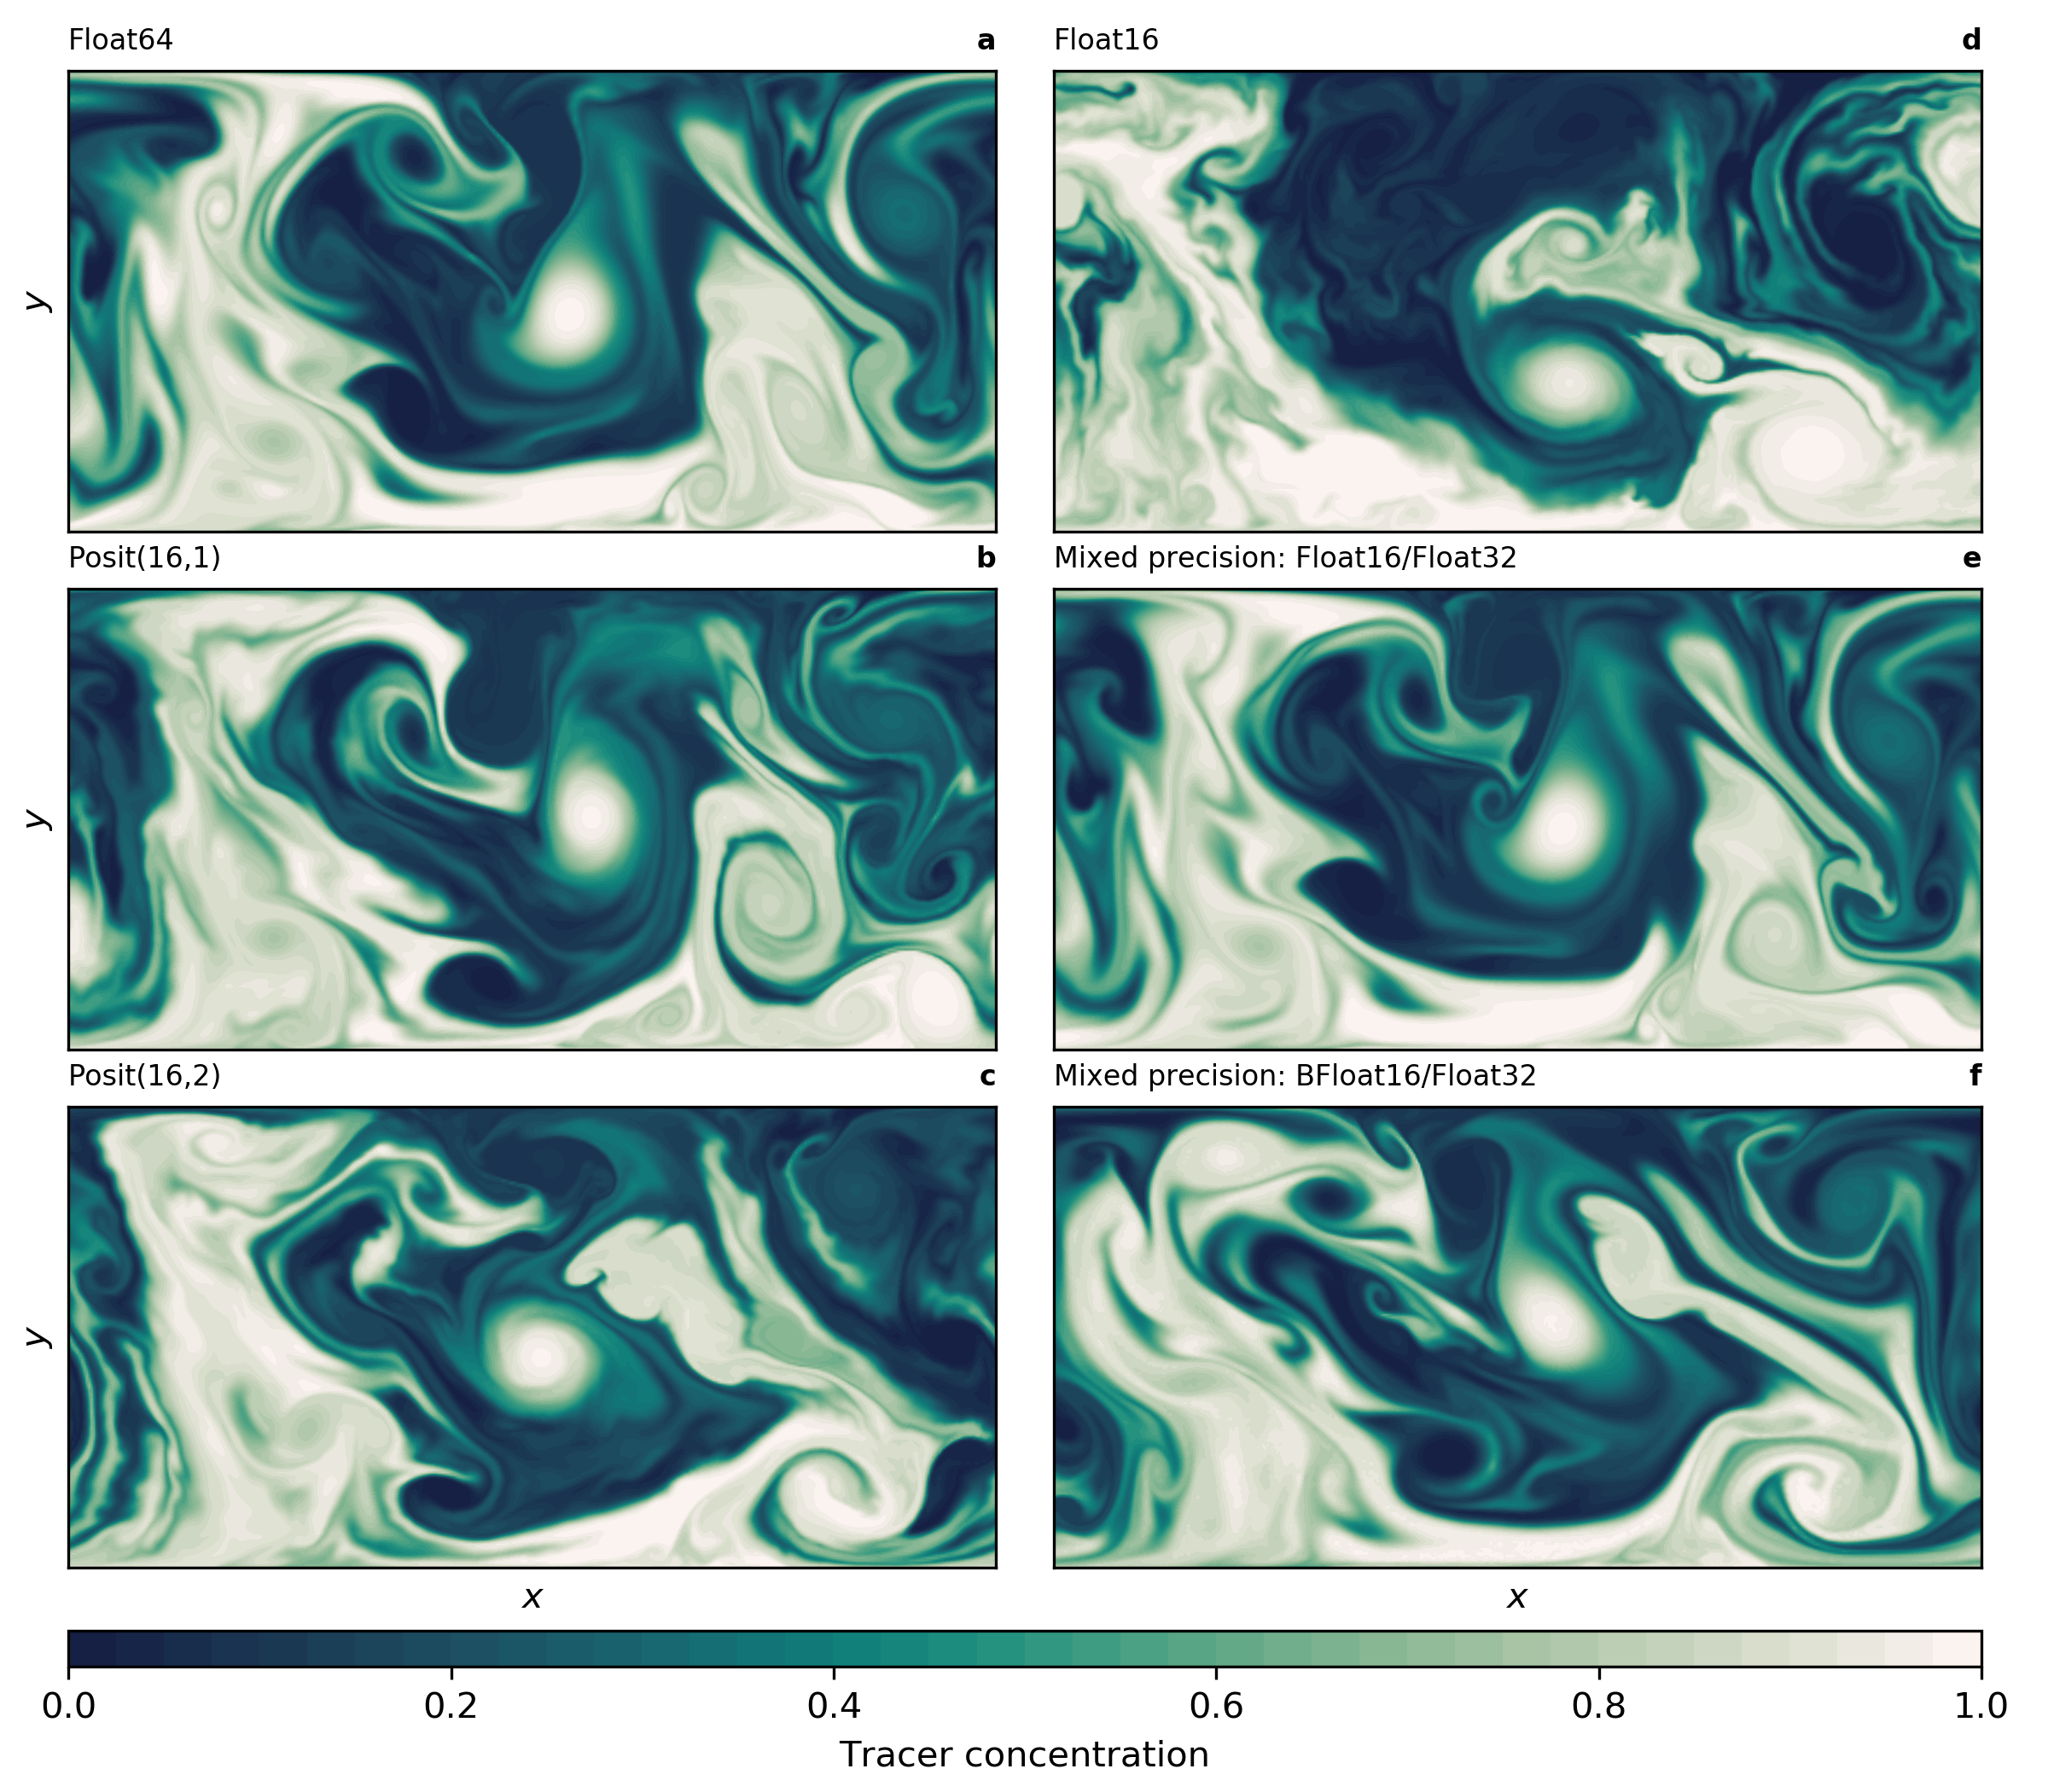
\includegraphics[width=1\textwidth]{Figures/swm/snapshot.png}
\caption{\textbf{Snapshot of tracer concentration simulated by the shallow water model using different 16-bit number formats.}
The high-resolution configuration ($\Delta = 5$km) is used with 400x200 grid points. The mixed precision simulations presented
in \textbf{e} and \textbf{f} use Float32 for the prognostic variables only. The tracer was injected uniformly in the lower half of the
domain 50 days before the time step shown.}
\label{fig:snapshot}
\end{figure}

However, if communication volume is an identified bottleneck in a given application, which is often the case in weather and
climate models, a reduction in computing time can be achieved with reduced precision communication. Reliable model simulations
might be possible with 16 or even 8-bit communication, which would result in a significant reduction in communication volume.
In general, various lossy and lossless data compression techniques can be used to reduce communication volume. Lossless
communication allows for bit-reproducible compression, but reductions in communication volumes are small due to many
high entropy mantissa bits (see also section \ref{sec:compression_methods_compression} and chapter
\ref{chap:compression} in general). We therefore restrict ourselves to lossy type conversions to Float16, Float8 or Posit8,
which introduce rounding errors to the data that is sent around while the overhead due to encoding before and decoding
after communication remains small.

\section{Impact of low precision on the physics}
\label{sec:swm_physics}

The shallow water model simulates vigorous turbulence interacting with a zonal current (Fig. \ref{fig:snapshot}). Both float and
posit arithmetic in 16 bit present very similar fluid dynamics in comparison to the Float64 reference. A snapshot of tracer
concentration many simulated days after initialisation reveals turbulent mixing of the tracer that is also well simulated with posits.
However, with Float16 the simulation deviates faster from the reference than with Posit(16,1) (also called Posit16, as 1 exponent
bit is the default configuration for 16-bit posits, see Table \ref{tab:formats}) and to a lesser degree with Posit(16,2).
This is  presumably due to larger rounding errors triggering the small scale instabilities visible in the snapshot as wavy
filaments and fronts. These instabilities are clearly triggered by Float16 arithmetics, but to a lower degree also visible for posits.
This provides some visual evidence that accumulated rounding errors are reduced with posits, especially Posit(16,1). BFloat16
arithmetic is not able to simulate the shallow water dynamics, as tendencies are too small to be added to the prognostic variables. 
Hence, a stalling of the simulated flow is observed. The results with mixed precision, i.e. using Float16/Float32 and BFloat16/Float32,
will be discussed in section \ref{sec:swm_results_mixed}.

\begin{figure}
\includegraphics[width=1\textwidth]{Figures/swm/rmse_eta_darker.pdf}
\caption{\textbf{Forecast error of sea surface height $\eta$ measured as root mean square error (RMSE) taking Float64 as reference.}
\textbf{a} Forecast error for various 16-bit number formats and mixed 16/32-bit simulations for which the prognostic variables
are kept in Float32. \textbf{b} Forecast error for reduced precision communication in 8 or 16 bit with various number formats used
for encoding, with Float64 used for all calculations. The communication of boundary values occurs at every time step
for the prognostic variables. The RMSE is normalised by a mean forecast error at very long lead times. Solid or dashed lines represent
the median of 200 forecasts per number format. The shaded areas of each model configuration denote the interquartile
range of the forecast experiments.}
\label{fig:rmse}
\end{figure}

\subsection{Error growth}

Short-term forecasts at medium-resolution ($\Delta = 10$km) are performed to analyse the differences between
different 16-bit arithmetics. To quantify the error growth caused by rounding errors with different arithmetics in a
statistically robust way, we create a number of forecasts with each member starting from one of 200 randomly picked
start dates from a 50-year long control simulation. The forecast error in the shallow water model is computed as the 
root mean square error (RMSE) of sea surface height $\eta$ with respect to Float64 simulations. Other variables yield
similar results. Each forecast is performed several times with the various number formats but from identical initial conditions.
The error growth caused by rounding errors is additionally compared to the error introduced by discretisation. A low-resolution
model configuration with $\Delta = 20$km is used to quantify a realistic level of discretisation error. The RMSE is normalised
by the climatological mean forecast error at very long lead times, which is the same for all model configurations. When the
normalised RMSE reaches 1 all information on the initial conditions is removed by the chaotic evolution of the shallow water
system.

The forecast error of Float16 is as large as the discretisation error and clearly larger than with 16-bit posit arithmetic (Fig. \ref{fig:rmse}a).
Both 16-bit posit formats, i.e. Posit(16,1) with 1 exponent bit and Posit(16,2) with two, yield a forecast error that is several times smaller
than Float16. The forecast error of 32-bit arithmetic is several orders of magnitude smaller and is only after 200 days as large as the
error for 16-bit arithmetic at short lead times of about 10 days. Also at 32 bit, posit arithmetic clearly causes smaller rounding
errors and therefore outperform floats.

\begin{figure}
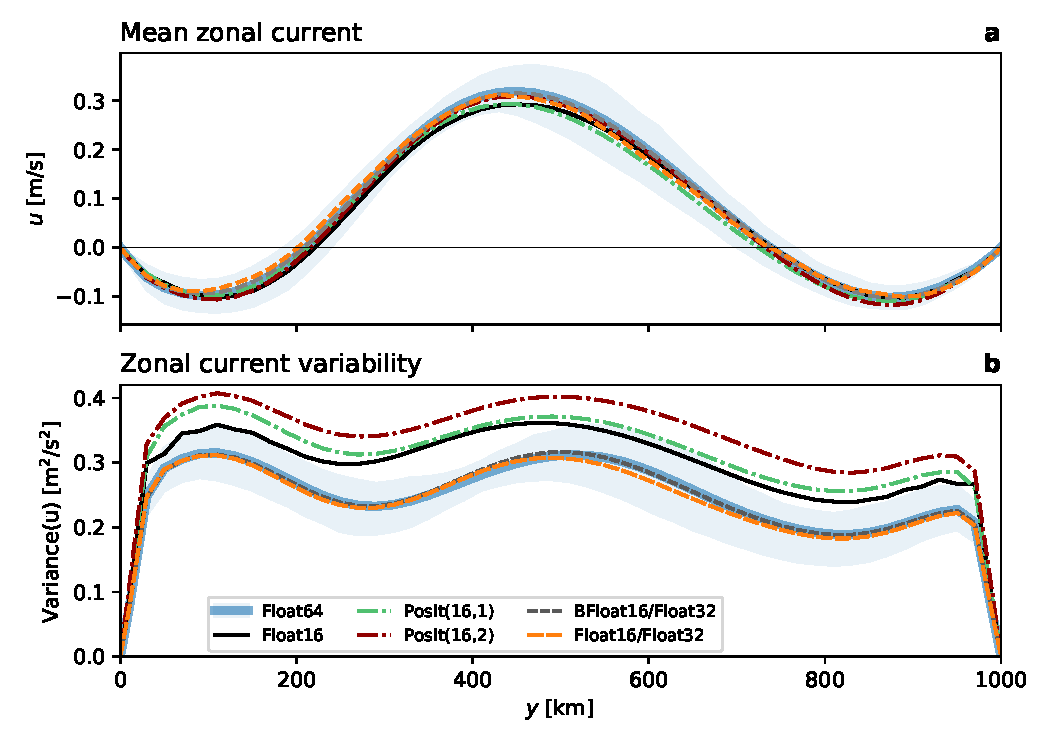
\includegraphics[width=1\textwidth]{Figures/swm/meanvar_u.pdf}
\caption{\textbf{Climatology and variability of the zonal current in the medium-resolution simulations.} \textbf{a} Zonally-averaged zonal
current $u$ as a function of the meridional coordinate $y$. \textbf{b} Zonal variance of the zonal current as a function of $y$. The dashed
lines for BFloat16/Float32 and Float16/Float32 are almost identical. The shaded area denotes the interquartile temporal variability around
the \textbf{a} mean and \textbf{b} variance of reference simulations with Float64.}
\label{fig:mean}
\end{figure}

\subsection{Mean and variability}

To investigate the effect of rounding errors on the climatological mean state of the shallow water system, we zonally average the zonal
velocity $u$. This average is based on 300-day long simulations starting from 200 different initial conditions, which cover the various
states in the long-term variability of the shallow water system. The climatology from a single very long simulation has not been assessed.

The mean state is an eastward flow of about 0.3~m/s, about 3 to 4 times weaker than instantaneous velocities throughout the domain
(Fig. \ref{fig:mean}a), which is typical for turbulent flows. A weak westward mean flow is found at the northern and southern boundary. 
No 16-bit format was found to have a significant impact on the mean state. The variability of the flow around its mean state is high
throughout the domain (Fig. \ref{fig:mean}b). The variability is significantly increased by 10 -- 30\% with 16-bit arithmetic, especially with
Posit(16,2). This is presumably caused by rounding errors that are triggering local perturbations which increase variability.

\begin{figure}
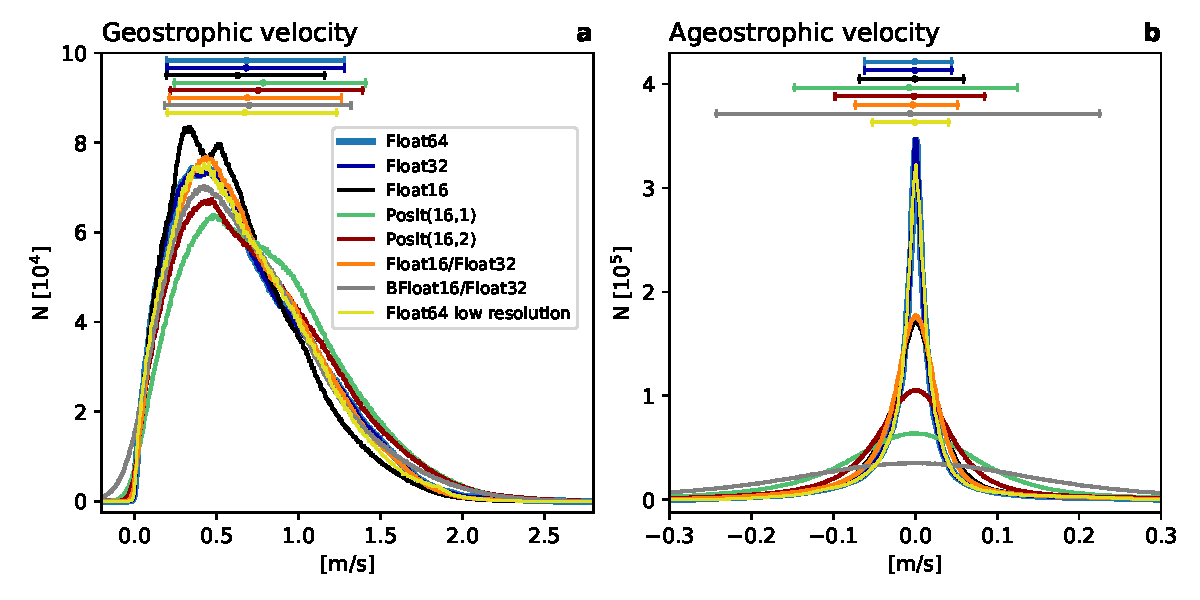
\includegraphics[width=1\textwidth]{Figures/swm/ageostrophic.pdf}
\caption{\textbf{Geostrophic balance as simulated with different number formats.}
\textbf{a} Histograms of flow-parallel components of geostrophic velocity. \textbf{b} as (a) but for the ageostrophic velocities, as
defined by Eq. \ref{eq:parallel}. Horizontal bars denote the mean, 10th and 90th-percentile in respective colours.}
\label{fig:geo}
\end{figure}

\subsection{Geostrophy}

The turbulence in shallow water simulations is largely geostrophic, such that the pressure gradient force opposes the Coriolis force.
The resulting geostrophic velocities $\mathbf{u}_g$ can be derived from the sea surface height $\eta$ as
\begin{subequations}
\begin{align}
\mathbf{u}_g &= \frac{g}{f}\hat{\mathbf{z}} \times \nabla \eta \\
\mathbf{u} &= \mathbf{u}_{g} + \mathbf{u}_{ag}
\end{align}
\label{eq:geo}%
\end{subequations}
and deviations from the actual flow $\mathbf{u}$ are the ageostrophic velocity components $\mathbf{u}_{ag}$. We project both
components on the actual velocities to obtain the flow-parallel components $\tilde{u}_{g}$ and $\tilde{u}_{ag}$ via
\begin{equation}
\tilde{u}_g = \frac{\mathbf{u}_g \cdot \mathbf{u}}{\| \mathbf{u} \|},
\quad \tilde{u}_{ag} = \frac{\mathbf{u}_{ag} \cdot \mathbf{u}}{\| \mathbf{u} \|}.
\label{eq:parallel}%
\end{equation}
The geostrophic velocities in the shallow water simulations can reach up to 2 m/s, are rarely negative (i.e. against the flow
$\mathbf{u}$) and have a mean of about 0.7 m/s (Fig. \ref{fig:geo}a). This behaviour is well simulated with 16-bit number
formats, although both 16-bit posit formats increase the mean of geostrophic velocities slightly. Ageostrophic velocity components
are found to be largely isotropic, and are therefore oriented equally frequent with and against the prevailing flow. They rarely exceed
$\pm$0.1m/s and are comparably small, as expected in geostrophically balanced turbulence. Ageostrophic velocities can be seen
as a measure of the physical instabilities in the flow field and their variance is indeed increased when simulated with 16-bit number
formats. Float16 and posits show clearly fewer ageostrophic velocities around 0, pointing towards an increased number of simulated
instabilities. Especially Posit(16,1) increases the variance of ageostrophic velocities by more than a factor of two. It is unclear where
in the model integration rounding errors of 16-bit arithmetic trigger instabilities that lead to the observed increase in ageostrophy.
We conclude that although the geostrophic balance in the simulations is maintained, rounding errors lead, likely due to an increase
in ageostrophy, to a higher variability in the flow field.

\begin{figure}
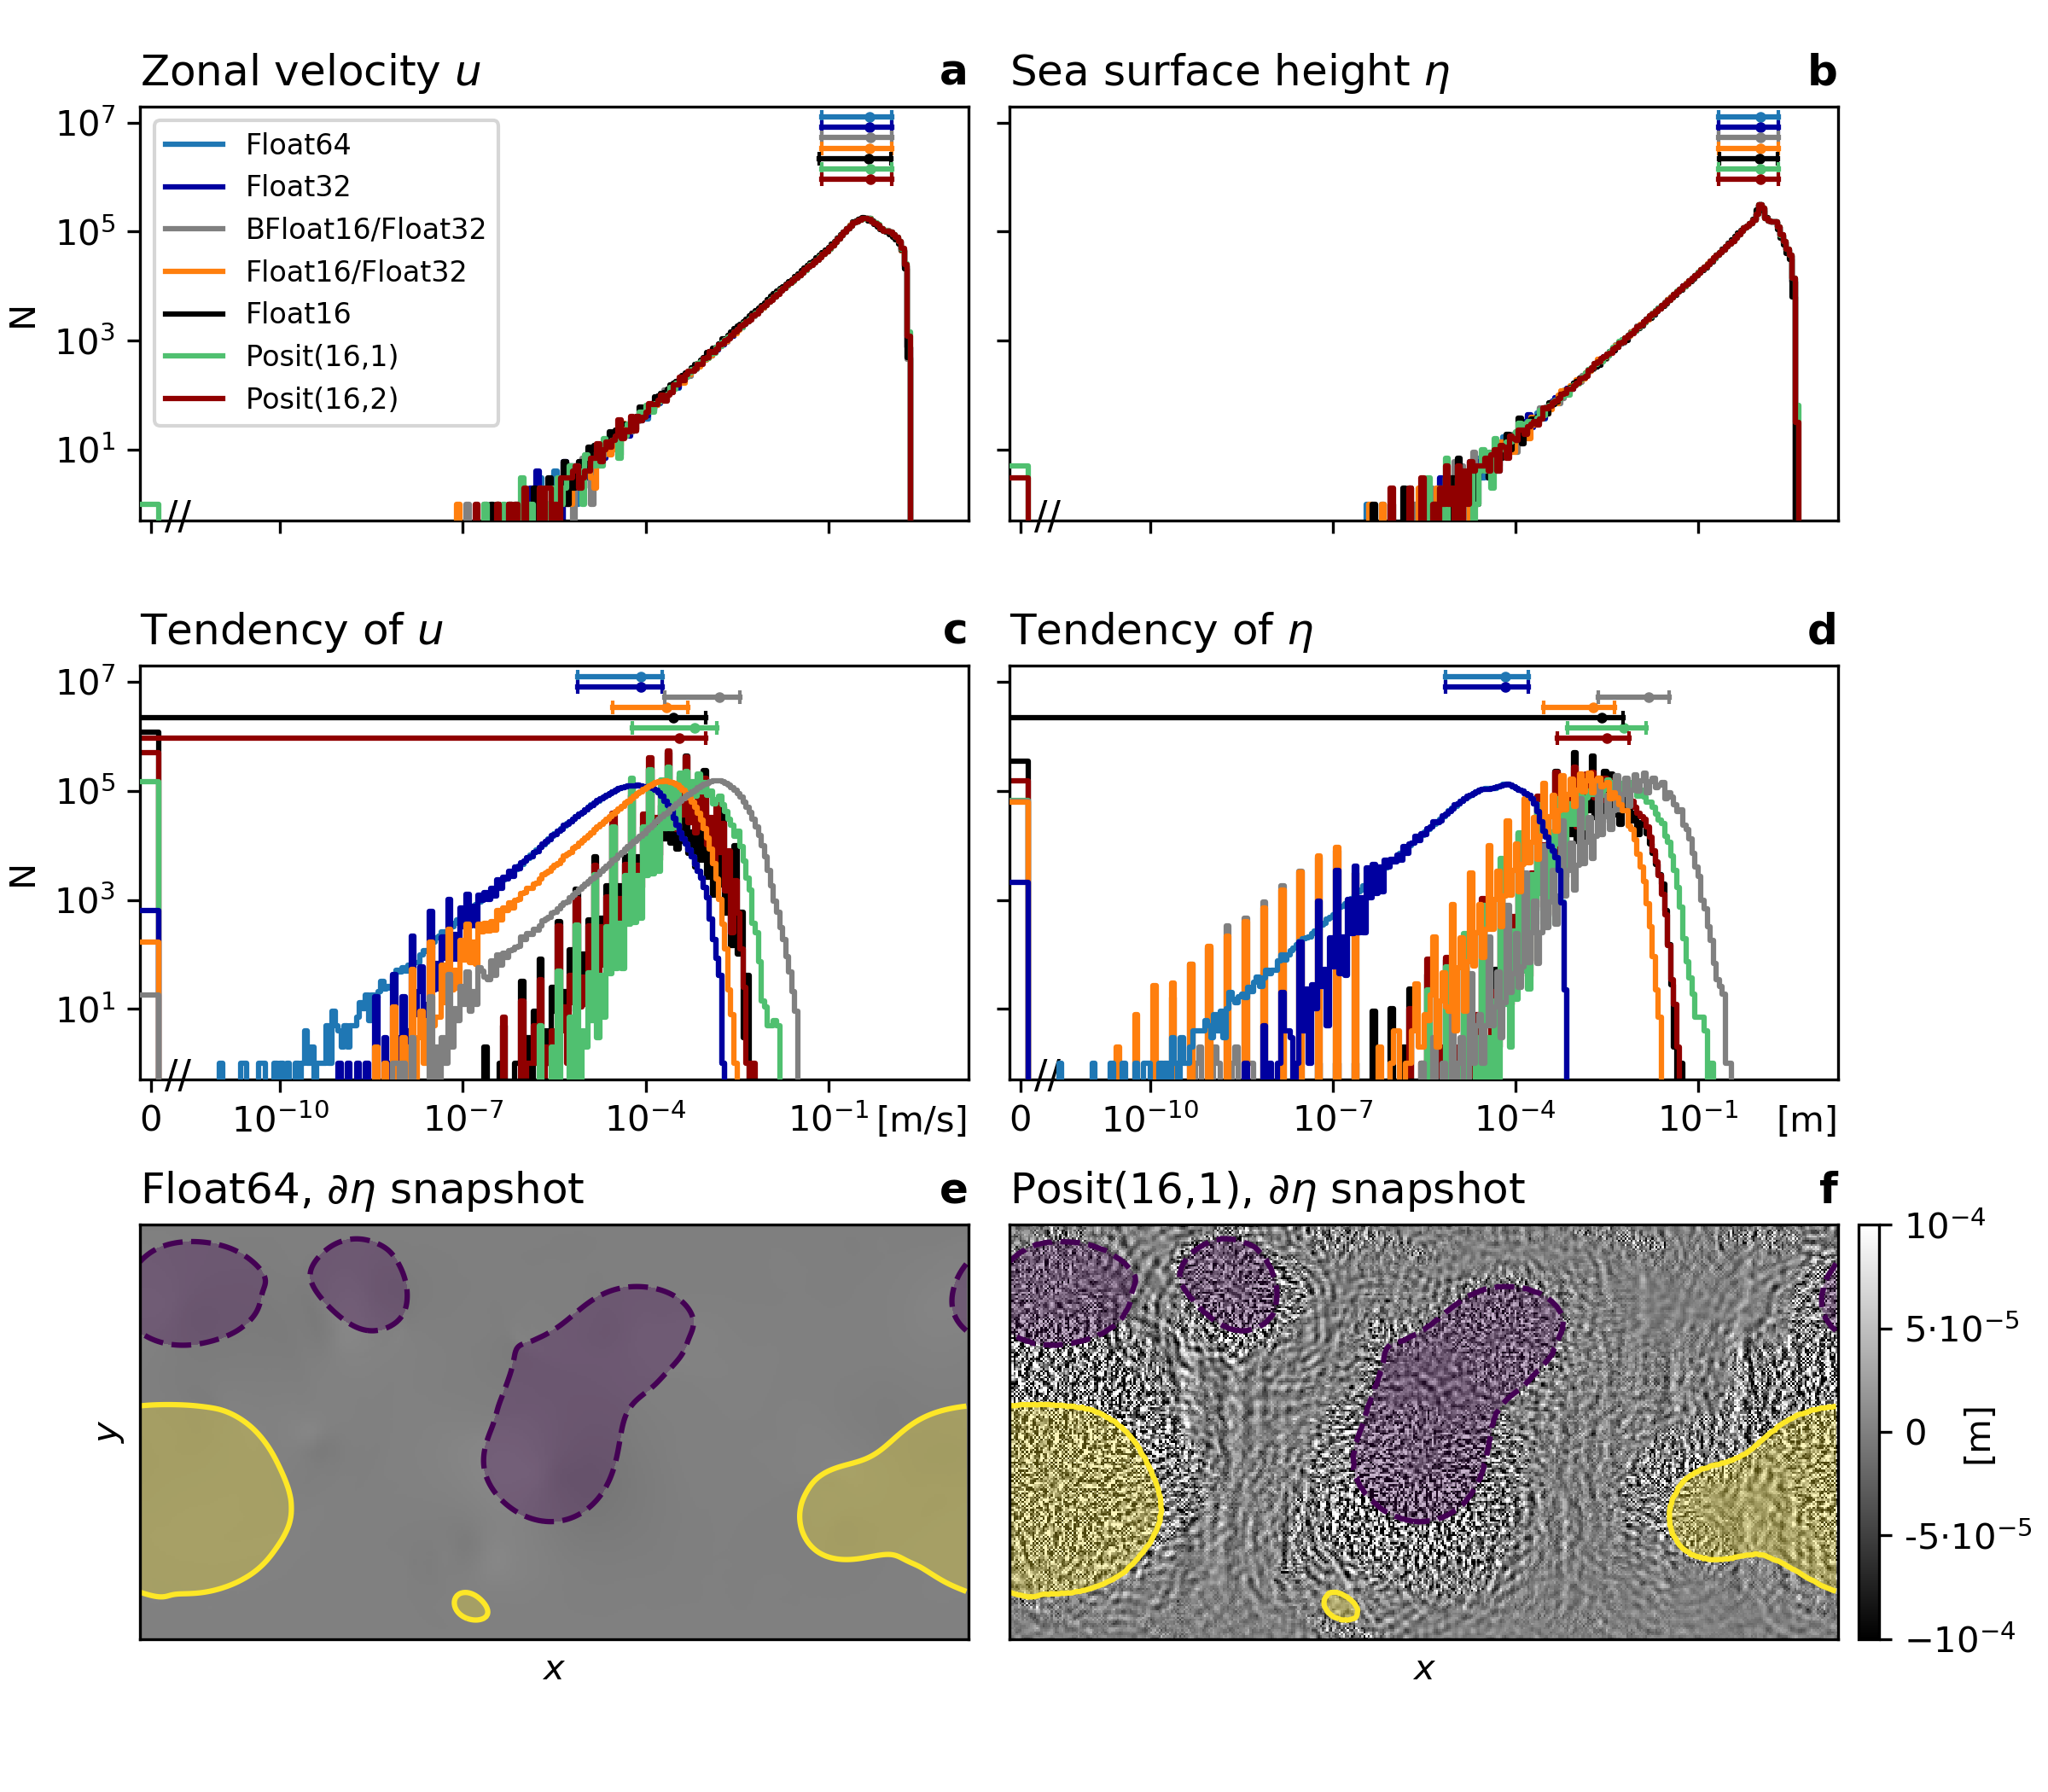
\includegraphics[width=1\textwidth]{Figures/swm/tendency_hist2.png}
\caption{\textbf{Detecting gravity waves due to rounding errors from low precision.} Histograms of the numeric values of the prognostic
variables \textbf{a} zonal velocity $u$, \textbf{b} sea surface height $\eta$, and the respective tendencies of \textbf{c} $u$ and
\textbf{d} $\eta$, simulated with different 16, 32 and 64-bit number formats. Mean, 10th and 90th percentile are shown above the
histograms in respective colours. Snapshots of the tendencies of $\eta$ simulated with \textbf{e} Float64 and \textbf{f} Posit(16,1).
Snapshots are similar for other 16-bit formats (not shown here). Areas of sea surface height anomalies exceeding $\pm1.4$~m are
shown in purple (negative) and yellow (positive). Note the break on the x-axis close to zero in \textbf{a-d}.}
\label{fig:tend}
\end{figure}

\subsection{Gravity waves}

As 16-bit arithmetics have no significant impact on the climatological mean state, histograms of prognostic variables are also not
changed (Fig. \ref{fig:tend}a and b). However, the tendencies are increased by orders of magnitude with 16-bit arithmetics
(Fig. \ref{fig:tend}c and d) as rounding errors cause gravity waves to radiate away from eddies (Fig. \ref{fig:tend}f). 
Gravity waves are identified from the tendency of sea surface height $\eta$. Comparing their propagation to the location of
anomalous sea surface height, which is used as a proxy to locate eddies, we assume that rounding errors in regions
of high eddy activity lead to instabilities that propagate away in the form of gravity waves. These gravity waves are not
present in Float64 simulations (Fig. \ref{fig:tend}e) and tend to have only a small impact on quasi-geostrophic dynamics,
as they act on different time and length scales. It is unclear but possible that gravity waves cause the observed increased
ageostrophic velocities for 16-bit arithmetic.

Tendencies are about 4 orders of magnitude smaller than the prognostic variables. This poses a problem for number formats
with a machine epsilon, measured as decimal precision, significantly lower than 4 decimal places (Table \ref{tab:formats}).
Float16 has a machine epsilon of 3.7, which is presumably close to the lower limit beyond which the addition of tendencies
will be round back. The BFloat16 number format has a machine epsilon of 2.8, which explains why flow is stalling when
simulated with BFloat16.

\subsection{Mixed-precision results}
\label{sec:swm_results_mixed}

In the previous simulations the entire shallow water simulation was performed with the specified number format. As the addition
of tendencies to the prognostic variables was identified as a key calculation that is error-prone, we investigate now the benefits
of mixed precision arithmetic, where Float32 is used for the prognostic variables but the tendencies are computed with either
Float16 or BFloat16, two number formats that have the lowest decimal precision around 1. The prognostic variables are now
reduced to Float16 or BFloat16 before the tendencies are calculated and every term of the tendencies is converted back before
addition to the prognostic variables. The continuity equation (Eq. \ref{eq:swe}b) then becomes
\begin{equation}
\frac{\partial \eta_{32}}{\partial t} = -\op{Float32}( \partial_x(u_{16}h_{16})
+ \partial_y(v_{16}h_{16} ))
\label{eq:conversion}
\end{equation}
and similar for $u$ and $v$ in Eq. \ref{eq:swe}a. Subscripts 16 and 32 denote variables held at 16 and 32-bit precision, respectively,
and Float32() is the conversion function.

Snapshots of tracer concentration reveal well simulated geostrophic turbulence (Fig. \ref{fig:snapshot}e and f) with Float16/Float32
and BFloat16/Float32 and instabilities at fronts or in filaments are visibly reduced compared to 16-bit arithmetic for all calculations.
The forecast error growth is strongly reduced once the prognostic variables are kept as Float32 (Fig. \ref{fig:rmse}a), supporting the
hypothesis that the addition of tendencies to the prognostic variables is a key computation with low rounding error-tolerance. Although
BFloat16 is not suitable for shallow water simulations when applied to all computations, mixing BFloat16 with Float32 yields a similar error
growth to posits, which is well below the discretisation error. Mean state or variability are virtually identical for both mixed precision cases
(Fig. \ref{fig:mean}) compared to the Float64 reference. The geostrophic balance is largely unaffected, but ageostrophic velocities
increase in variance, especially for BFloat16 (Fig. \ref{fig:geo}). Gravity waves are similarly present for mixed precision although weaker
for tendencies computed with Float16 (Fig. \ref{fig:tend}d) and, as discussed, they tend to not interact with the geostrophic time and
length scales. Although the results show that Float16 is generally a preferable number format over BFloat16 for the applications presented
here, we acknowledge that the conversion between Float32 and Float16 will come with some computational cost. In contrast, the
conversion between BFloat16 and Float32 is computationally very cheap as both formats have the same number of exponent bits.
Removing significant bits, applying rounding, and padding trailing zeros, are the only operations for this conversion. Following the
results here, mixing 16 and 32-bit precision is found to be an attractive solution to circumvent spurious behaviour due to 16-bit
floating-point arithmetics. Performance benefits are still possible as most calculations are performed with 16 bit, with error-critical
computations in 32 bit to reduce the overall error.

Using mixed-precision in our shallow water model, 77\% of the arithmetic operations are performed in 16 bit and the remaining
23\% in 32 bit. Assuming Float16/BFloat16 to be two times faster than Float32 and conversion costs to be negligible this would
yield another 40\% reduction in computing time on top of a reduction from Float64 to Float32. However, this depends on the soft
and hardware implementation considered. Some of the 16-bit accelerators (GPU/TPU) can increase the flop rate by more than a
factor of 2 when compared to Float32. In addition, the shallow water model regarded here has a comparably simple right-hand side,
such that more complex models will spend more time to compute tendencies which will come with a larger performance increase.

Mixed-precision is an attractive solution as hardware-accelerated 16-bit floating-point arithmetic is already available on graphic or
tensor processing units and implementations therefore do not rely on the development of future computing hardware, which is the
case for posits.

\begin{figure}
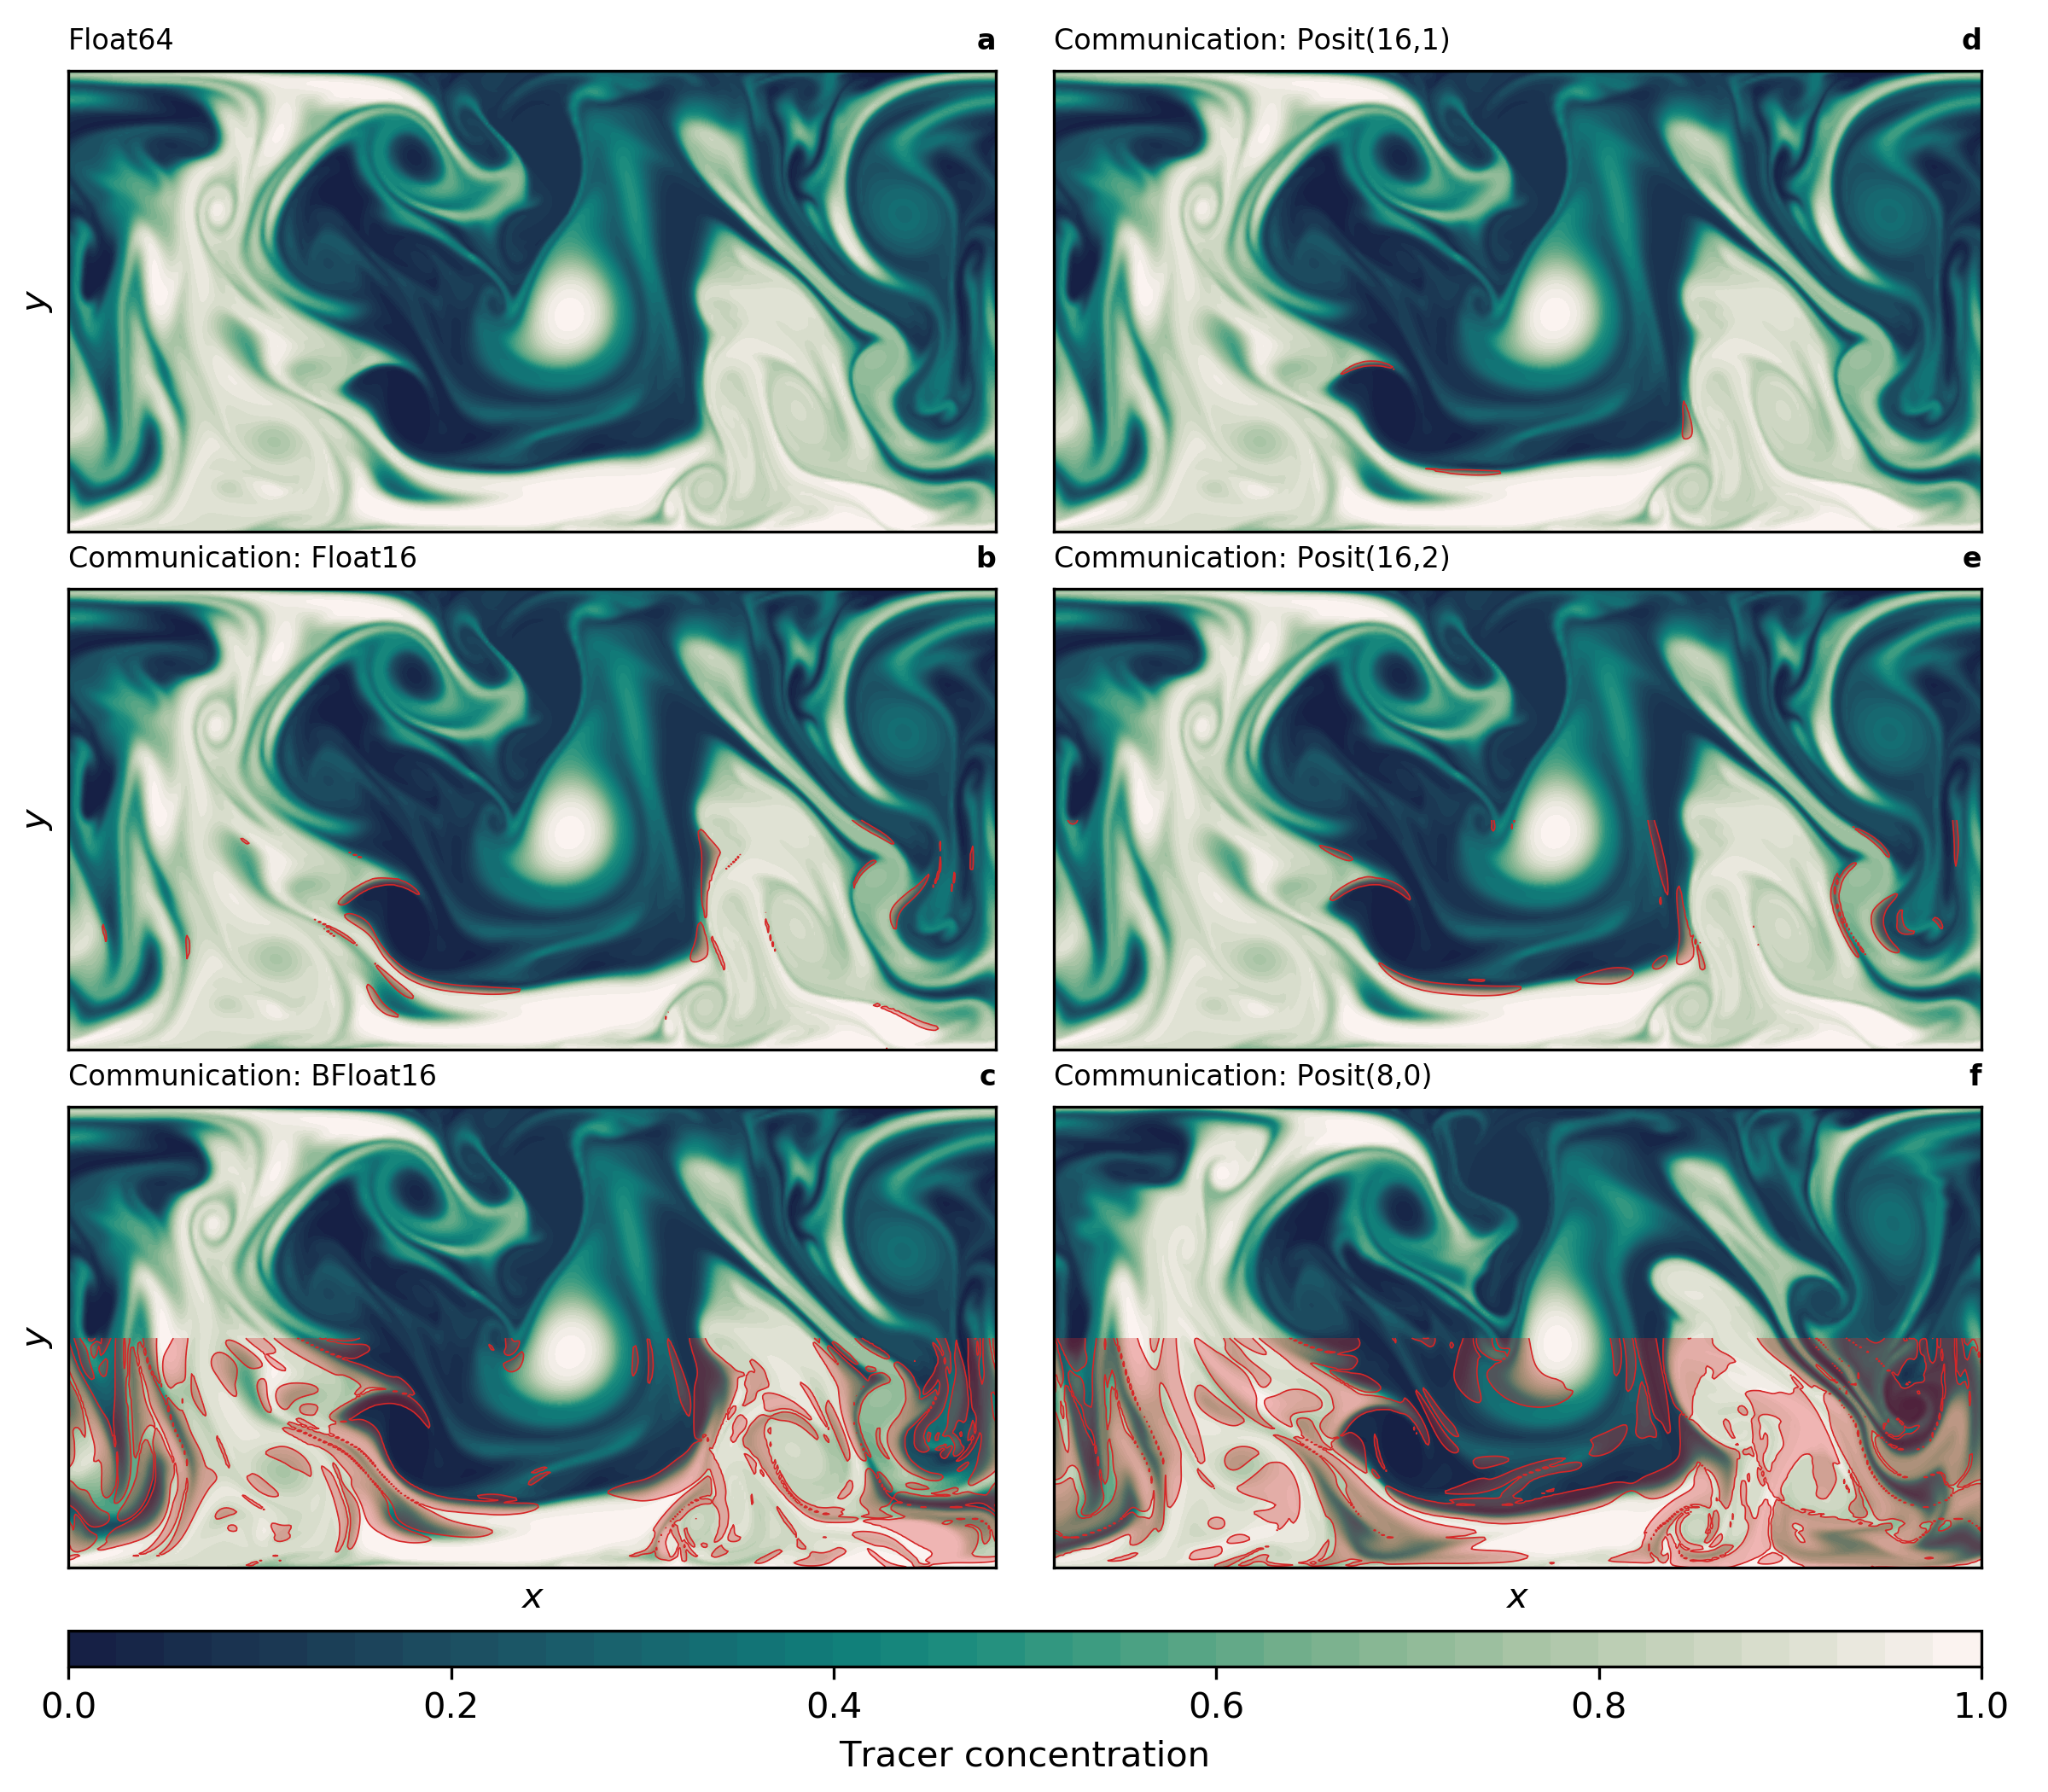
\includegraphics[width=1\textwidth]{Figures/swm/snapshot_comm.png}
\caption{\textbf{Snapshot of tracer concentration simulated by the shallow water model using reduced precision communication.}
The communication of boundary values occurs at every time step for the prognostic variables. Float64 was used for all calculations.
Areas where the absolute error exceeds 0.05 are shaded in red only in the lower half of the domain. The tracer was injected uniformly
in the lower half of the domain 50 days before. This simulation was run in the high-resolution configuration ($\Delta = 5$km).}
\label{fig:snapshot_comm}
\end{figure}

\subsection{Reduced-precision communication results}
\label{sec:swm_results_comm}

A standard method to parallelise simulations is the distributed-memory parallelism via Message Passing Interface (MPI, \cite{TheMPIForum1993}).
We emulate MPI-like communication in the shallow water model with the copying of boundary values between the right and left boundary (periodic
boundary conditions). Although the shallow water model does not run in parallel, reducing the precision in the copying of boundary values
introduces an equivalent error as if reduced precision MPI communication was used between subdomains. Reduced precision is applied
for the communication of the prognostic variables at every Runge-Kutta substep.

Regarding snapshots of tracer concentration simulated with reduced precision communication shows a negligible error for Float16 and
16-bit posits (Fig. \ref{fig:snapshot_comm}). The error is largest at fronts and not concentrated around the boundaries. Encoding the
communication with BFloat16 introduces a larger error than for the other 16-bit formats as the decimal precision is with 2.8 clearly lower
(Table \ref{tab:formats}) for the range of values occurring within the prognostic variables (Fig. \ref{fig:tend}a and b). The errors are quantified
by the RMSE of surface height $\eta$ as before and are up to about two orders of magnitude smaller than the errors that result from 16-bit arithmetic.
Even the worst format for 16-bit communication, BFloat16, has a smaller error than the best mixed precision formats, Float16 with Float32.
We therefore extend the short-term forecast experiments to include two 8-bit formats, Posit(8,0) and Float8 (see Table \ref{tab:formats} for
a description). Both formats are found to be suitable for reduced precision communication here and do not introduce an error that is larger than the
discretisation error. Having said that, Float8 communication introduces an error that is comparably large in the first days but growths only
linearly in the first 50 days of the simulation, which is in contrast to the exponential error growth observed for 16-bit arithmetic.

\section{Discussion}
\label{sec:swm_discussion}

Future high-performance computing architecture will increasingly support 16-bit arithmetics. The wall-clock time for weather and climate
simulations could be greatly reduced if computationally demanding algorithms were run at such reduced precision. We tested a number
of options for 16-bit arithmetic for weather and climate applications in a shallow water model. The best results were achieved with 16-bit
posits which appear very promising for application in high-performance computing for Earth System modelling. Float16 can be used to
perform forecasts with the shallow water model while the application of BFloat16 was not successful.

In general, 16-bit arithmetics were not found to alter the climatological mean state or the large-scale dynamics. However, 
variability and ageostrophic velocities were increased, such that second and higher-order statistics should undergo testing
to assess the models reliability. Depending on the application, an increased variability does not  necessarily deteriorate the
model, especially for more realistic model set-ups than considered here. However, our findings suggest that reduced-precision
changes need to be done carefully as specific simulation features can change without obvious impact on mean diagnostics.

Shallow water simulations with 16-bit arithmetic required rescaling of some terms but no major revisions of the model code
or algorithms. Given that only floats are currently hardware-supported, we investigated mixed-precision approaches.
Keeping the prognostic variables at 32 bit while computing the tendencies in 16 bit reduced the rounding errors significantly.
We also showed that numerical precision for communication between compute nodes can be greatly reduced down to 16 or
even 8-bit without introducing a large error. Reduced precision communication was not found to have a significant impact on
either mean state, variability, geostrophy or tendencies.

A \emph{perfect model} is used in this study, such that any form of model or initial condition error is ignored and only the number
format is changed between simulations. Solely discretisation errors are estimated by lowering the spatial resolution by a factor of 2.
Although this is essential here to analyse the impact of rounding errors isolated from other errors, it is in general not a realistic
configuration for weather or climate models. More complex models include many other sources of forecast error, such that the
contribution of rounding errors from 16-bit arithmetic would likely be dwarfed by model, discretisation or initial condition errors.

Only the most common discretisation method for fluid dynamics was used in this study: Finite differences with an explicit time
stepping scheme. But various other discretisation methods exist, such as finite element or volume, spectral methods and
implicit time stepping. These methods come with different algorithms and associated precision requirements. Consequently,
some might be less tolerant to rounding errors than the method used in this study.

There is currently no hardware available for posit arithmetic that we could have used for performance testing and it is seems
impossible to make credible estimates whether such hardware would be faster or slower when compared to hardware optimised
for Float16 arithmetic (as this does not only depend on theoretical considerations but also on investments into chip design).
We therefore cannot draw any conclusion about the performance of posit arithmetic operations in comparison to Float16 or
the other formats.

Until progress is made on hardware implementations for posits, the results here suggest that also 16-bit float arithmetic can
successfully be used for parts of complex weather and climate models with the potential for acceleration on graphic and tensor
processing units. It is therefore recommended to adapt a type-flexible programming paradigm, ideally in a language that supports
portability, with algorithms written to reduce the dynamic range of arithmetic results. Hardware progress on central, graphic or
tensor processing units, with various numbers formats supported, can subsequently be utilised to accelerate weather and
climate simulations.
